%intro%

The best theoretical model we currently have that describes all the known fundamental particles and their interactions is known as the standard model.
%The standard model (SM) of particle physics is the best theoretical model we currently have that describes all the known fundamental particles and their interactions.
This chapter will reviews the basics of the Standrad Model (SM). (update when the content of chapter is compelet)

%..........................
%\section{The Standrad model}

Particles in the SM can be classified into two categories, as shown in Fig.~\ref{fig:SMParticles}, based on their spin (intrinsic angular momentum) value: fermions have half integer spin, bosons have full integer spin.

Fermions include particles that make up matter: electrons, protons, and neutrons. All fermions follow the Pauli exclusion principle which is essential for building atoms and the periodic table. This group of particles can be divided further into two groups based on the strong force: leptons, which do not undergo strong interactions, and quarks, which have strong nuclear interactions.

Quarks cannot be isolated because of the color confinement. They are always found in a bound state known as hadrons interacting via strong force.
%KH Hadrons either composed of three quarks, baryons, or a pair of a quark and anti-quark, mesons. Baryons have half integer spin so they are considered fermions while mesons have integer spin so they are considered bosons.
Hadrons are classified into two categories: baryons and mesons.
Baryons consist of three quarks, while mesons are composed of a quark-antiquark pair.
Baryons have a half-integer spin, making them fermions, whereas mesons possess an integer spin, classifying them as bosons.

The leptons group consists of three electrically charged particles (electron, muon, and tau) and three electrically neutral neutrinos that come in three flavors associated with the electron, muon, and tau. The electrically charged leptons interact with all forces except for the strong force, while neutrinos only interact through gravity and weak force.

Both quarks and leptons can be categorized into
%Each group in quarks  and leptons can be organized into
three generations that differ in their mass.
The heavier generation can decay into the lighter generation
until they reach the lighter more stable particles such as electron, and up and down quarks.
%KenH till we reach the lightest one that is stable like (electron, up and  down quarks) (fix me) %“Here insert table that shows these generations”

The force carrying particles in the SM are vector bosons with spin 1. The electromagnetic force is carried by the photon. The strong force is carried by eight types of gluons. The weak interaction is carried by two charged W bosons and one neutral Z boson.
The Higgs boson is a spin-0 scalar particle responsible for imparting mass to other particles through interactions governed by the Higgs mechanism (see Fig.~\ref{fig:SMinteractions}).

% note:check if sm details are missing from draft1, also add figures

% include anti matter and how is it associated with matter particles check J.notes purple highlight) 
% use the SM figure
% maybe breifly mention the sectors of SM this is : QCS, EW , strong 
%(consider adding the shortcoming of the SM and how those reasons motivatin the directon of the HEP)
% why SM is incomplete? gravit? 
%..........................     

\begin{figure}[t!]

\centering
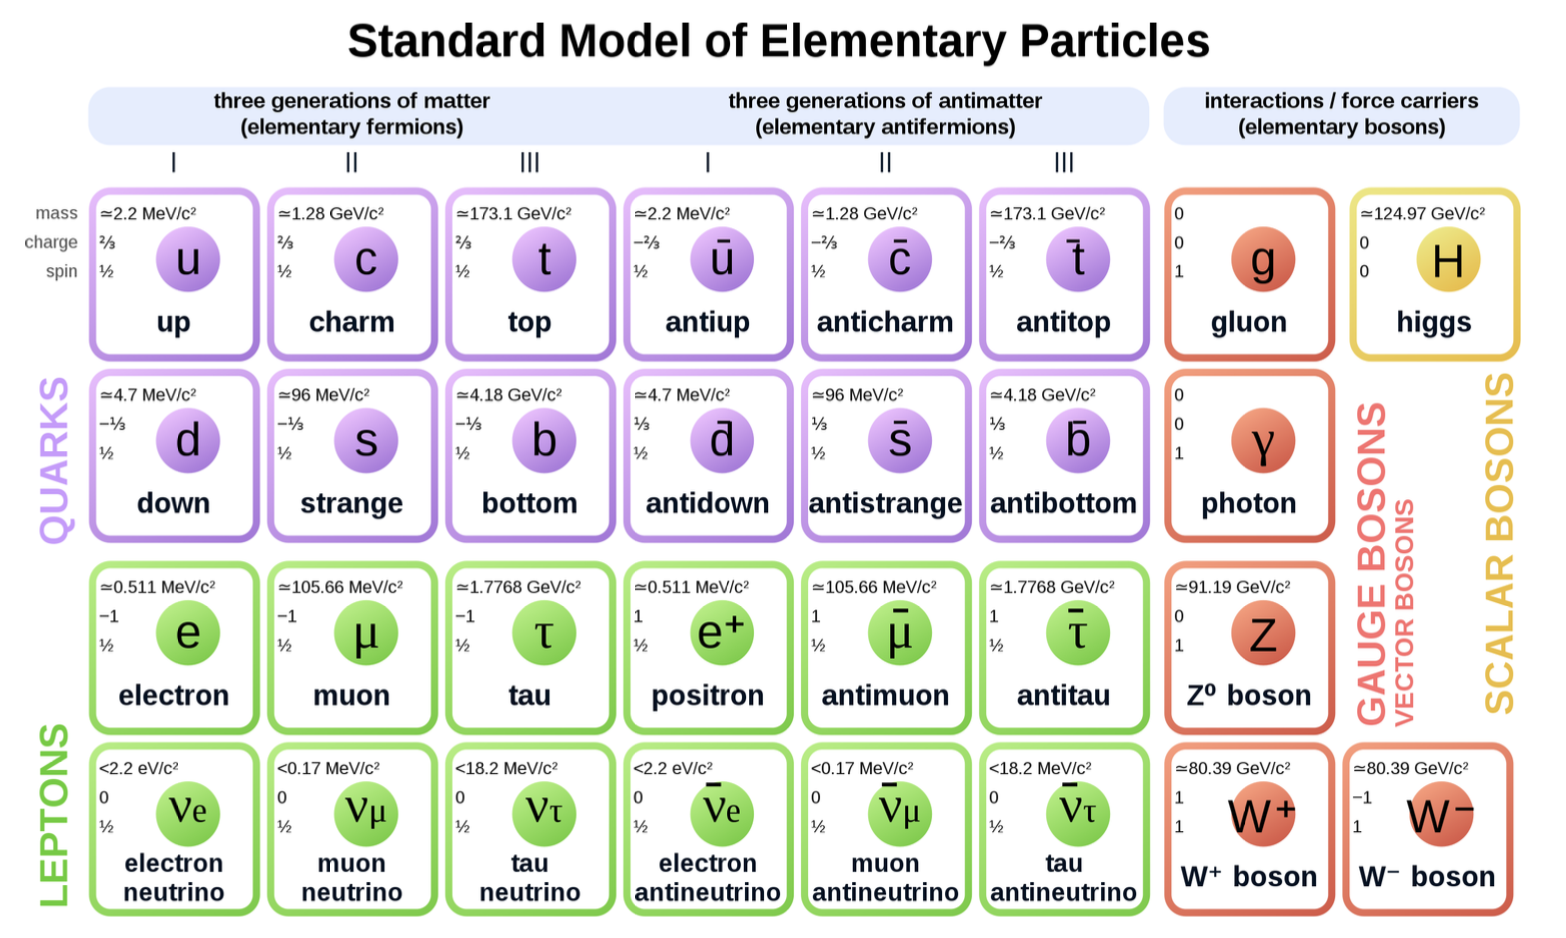
\includegraphics[width=0.99\textwidth]{figures/SM_include_antimatter.png}}
\caption[Summary of standard model fundamental particles]{Summary of SM fundamental particles. Figure source~\cite{SMtable}.
\label{fig:SMParticles}}

\end{figure}

\begin{figure}[t!]
\centering
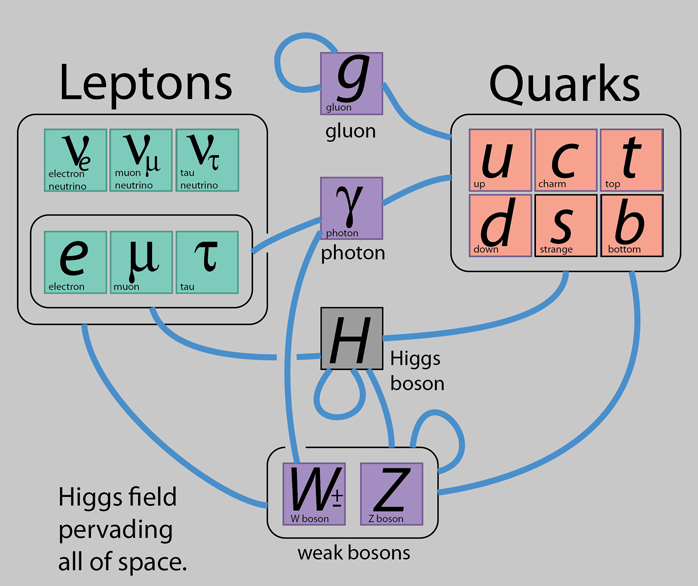
\includegraphics[width=0.99\textwidth]{figures/interactions_SM.png}}
\caption[Summary of standard model fundamental particles]{Summary of SM fundamental particles. Figure source~\cite{SMintera}.
\label{fig:SMinteractions}}
\end{figure} 
